\label{last}
\section{Introduction}
The algorithms described above were implemented in C++. For graph operations, the NetworKit and Koala libraries were used. The code is open source and available in the Koala-NetworKit GitHub repository at 
\url{https://github.com/krzysztof-turowski/koala-networkit/pull/23}.

\section{Implementation details}
The repository contains separate classes for each type of problem, such as cograph recognition, treewidth calculation, maximum clique calculation, and so on. Below is a brief description of the files with their purposes.
\begin{itemize}
    \item \texttt{koala-networkit/include/recognition/CographRecognition.hpp}

    The main header file defining the cograph recognition class.

    \item \texttt{koala-networkit/include/recognition/cograph/Part.hpp}
    
    Header file for the class implementing the Part and Element classes used by the recognition algorithm.
    
    \item \texttt{koala-networkit/include/recognition/cograph/FactorizingPermutation.hpp}
    
    Header file for the class implementing the creation and manipulation of a factorizing permutation. For example, adding or removing parts or elements, moving elements to different parts, and so on. It is used in the factorizing permutation construction algorithm.

    \item \texttt{koala-networkit/include/recognition/cograph/Twins.hpp}
    
    Header file for the class implementing operations with twin vertices in a cograph. For example, checking if vertices are twins. It is used in the single permutation testing algorithm.

    \item \texttt{koala-networkit/include/structures/Cotree.hpp}

Header file for the class implementing operations on the cotree and its vertices.
\item \texttt{koala-networkit/include/pathwidth/CographPathwidth.hpp}

Header file for the class implementing the calculation of graph pathwidth.
\item \texttt{koala-networkit/include/coloring/CographVertexColoring.hpp}

Header file for the class that finds the graph coloring with the minimum number of colors.

\item \texttt{koala-networkit/include/independent\_set/CographIndependentSet.hpp}

Header file for the class that finds the independent set of a graph.
\item \texttt{koala-networkit/include/max\_clique/CographMaxClique.hpp}

Header file for the class that finds the maximum clique of a graph.

\item \texttt{koala-networkit/benchmark/}

Folder containing benchmarking programs to evaluate the performance of the algorithms on various graph instances.

\item \texttt{koala-networkit/test/}

Folder containing unit tests for checking correctness of the implemented algorithms.

\end{itemize}
\section{Testing}
The correctness of each algorithm was tested in two ways:
\begin{enumerate}
    \item Unit tests on all small-sized graphs, i.e.  graphs with less than $15$ vertices. 
    \item On graphs from the benchmark containing random cographs and non-cographs with less than $10^6$ vertices.
\end{enumerate}

The following iterative algorithm generates random cographs. First, create $n$ cographs, each consisting of a single vertex. At each step, select and merge two random cographs into one. Then, with a given probability $p$, replace the cograph with its complement. The algorithm stops when all cographs merge into one. This algorithm can produce any cograph with $n$ vertices. At step $i$, merge cographs $G_i^1$ and $G_i^2$. 
Let the set $B_{x,y}=\{i \colon x,y \in (G_i^1 \cup G_i^2)\}$ include all the steps in which vertices $x$ and $y$ participated in the merging. Vertices $x$ and $y$ become neighbors if and only if the number of times the complement is used during these operations is odd. The probability of this is $1-\sum\limits_{i=0}^{|B|/2} \binom{|B|}{2 \cdot i}$. This fact allows generating graphs with a specific number of edges. For example, if $p=\frac{1}{2}$, then the probability of an edge existing between any pair of vertices is $\frac{1}{2}$. This follows from the well-known fact that forall n it is true that $\sum\limits_{i=0}^{i=n} {(-1)}^i \cdot \binom{n}{i}=0$.

\section{Running time}

The explanations of the algorithm names are provided in \Cref{tab:algorithms_number}.
The algorithms were tested on several subgroups of tests. 
Each test consists of 5 random graphs generated with the same number of edges and vertices. The average runtime, in milliseconds, are presented in \Cref{tbl:algorithms} and \Cref{tbl:algorithms1}. 



\begin{table}[]
    \centering
    \begin{tabular}{ | c | p{4cm} |}
  \hline
  Id & Algorithm \\ [0.5ex] 
  \hline\hline
  $A1$ &  Cograph recognition \\
  \hline
  $A2$ &  Independent set  \\
  \hline
  $A3$ &  Max clique \\
  \hline
  $A4$ &  Pathwidth \\
  \hline
  $A5$ &  Vertex coloring \\
  \hline
  \end{tabular}
  \caption{The algorithms numbers with their identifiers}
    \label{tab:algorithms_number}
\end{table}

  
\begin{table}[ht]
\centering
\begin{tabular}{ | c | c | c |}
\hline
$n$ & $m$ & $A1$    \\ [0.6ex] 
 \hline
 $10^3$ & $5 \cdot 10^3$ & 2  \\ [0.6ex] 
\hline
 $7*10^4$ & $10^5$ & 7100  \\ [0.6ex] 
  \hline
 $10^5$ & $2 \cdot 10^6$ & 49000  \\ [0.6ex] 
 \hline
 $10^6$ & $4 \cdot 10^7$ & $17 \cdot 10^5$  \\ [0.6ex] 
 \hline
\end{tabular}

\caption{The running time of the cograph recognition algorithm}
\label{tbl:algorithms}
\end{table}


\begin{table}[ht]
\centering
\begin{tabular}{ | c | c | c | c | c | }
\hline
$n$ & $A2$ & $A3$ & $A4$ & $A5$   \\ [0.6ex]
\hline
$10^5$ & 3 & 15 & 5 & 12 \\ [0.6ex] 
\hline
$5 \cdot 10^5$ & 16 & 108 & 26 & 90 \\ [0.6ex] 
\hline
$10^6$ & 33 & 238 & 53 & 189 \\ [0.6ex] 
\hline
$4 \cdot 10^6$ & 144 & 1369 & 212 & 910 \\ [0.6ex] 
\hline
$8 \cdot 10^6$ & 292 & 3157 & 425 & 2079 \\ [0.6ex] 
\hline
$2 \cdot 10^7$ & 732 & 9584 & 1105 & 6039 \\ [0.6ex]
\hline
$5 \cdot 10^7$ & 1993 & 28287 & 2741 & 18316 \\ [0.6ex]
\hline

\end{tabular}

\caption{The running time of different algorithms on cographs}
\label{tbl:algorithms1}
\end{table}


\section{Conclusions}

It is clear that the number of edges in the graph does not affect the performance of algorithms $A2, A3, A4, A5$. This is because these algorithms do not operate on the original cograph, but only on the constructed cotree. The algorithm from \Cref{Cotree construction} always constructs a cotree with $O(n)$ edges. The \Cref{fig:milliseconds} shows that these algorithms run in linear time and, within the tested range.

\begin{figure}[h!]
  \centering
  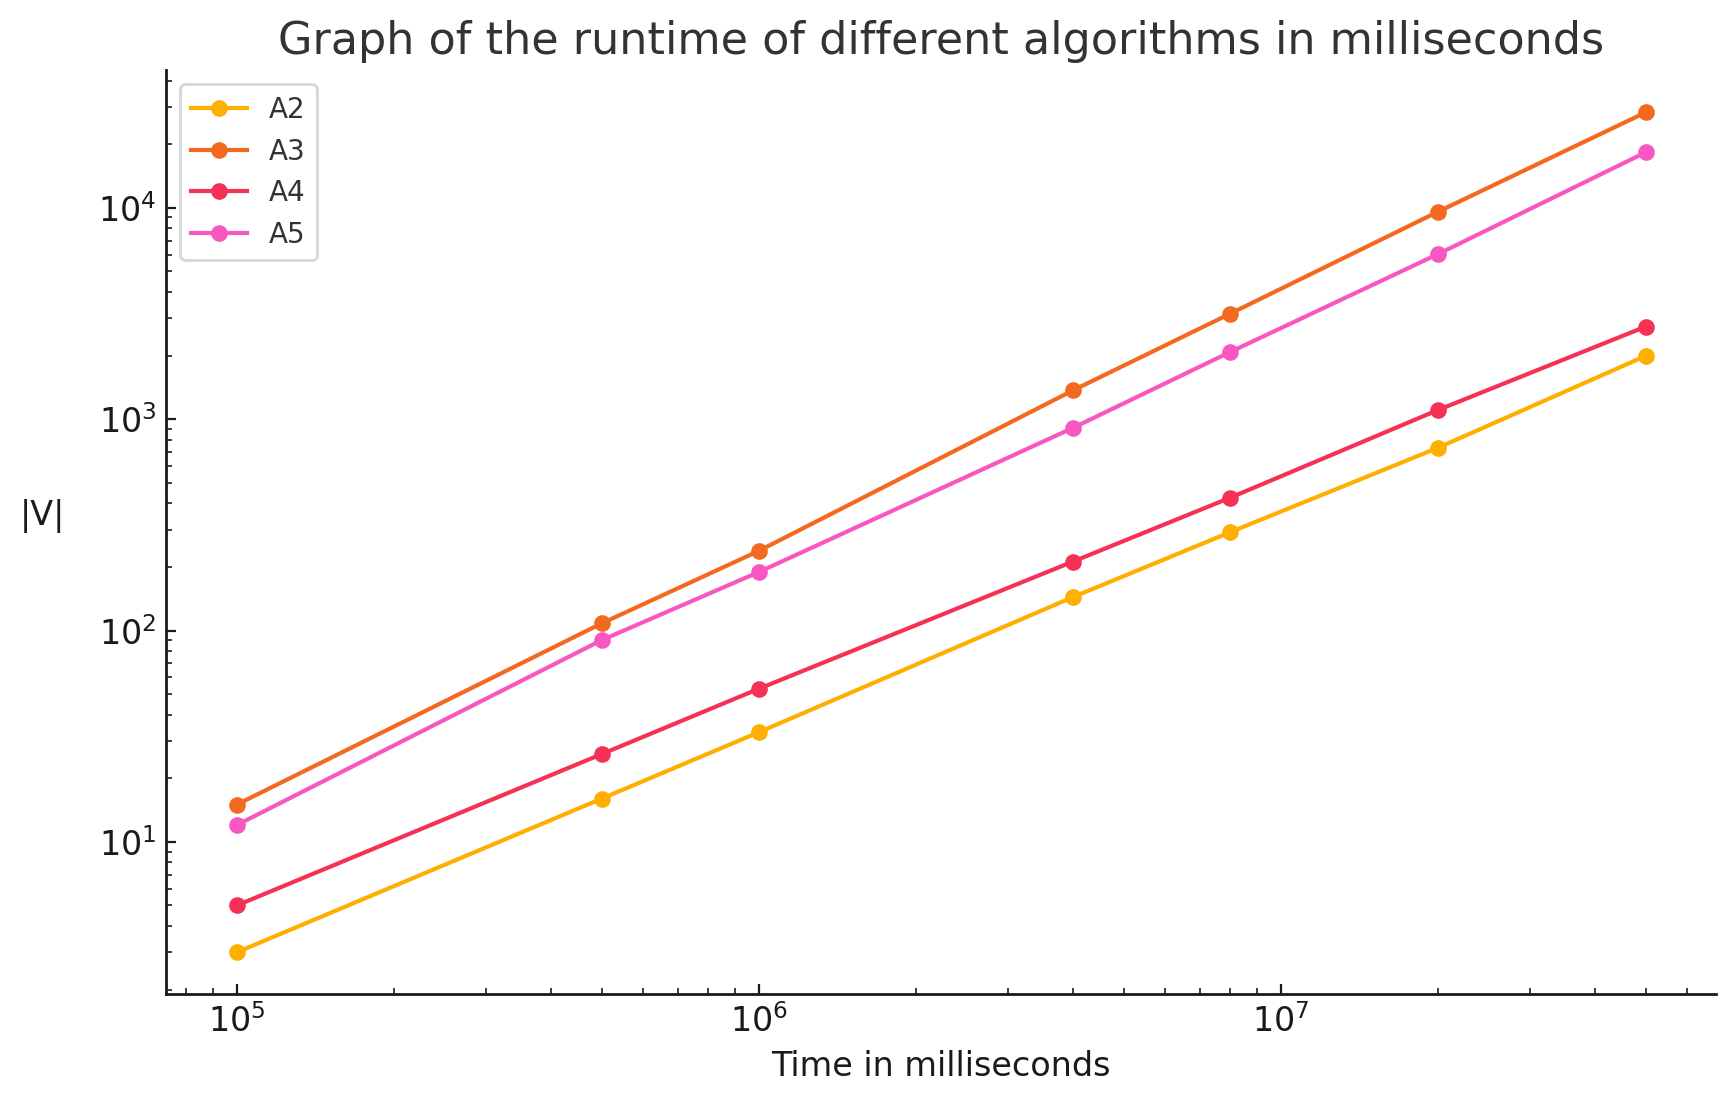
\includegraphics[width=\linewidth]{output (3).png}
  \caption{Graph of the runtime of different algorithms in milliseconds.}
  \label{fig:milliseconds}
\end{figure}


\begin{figure}[h!]
  \centering
  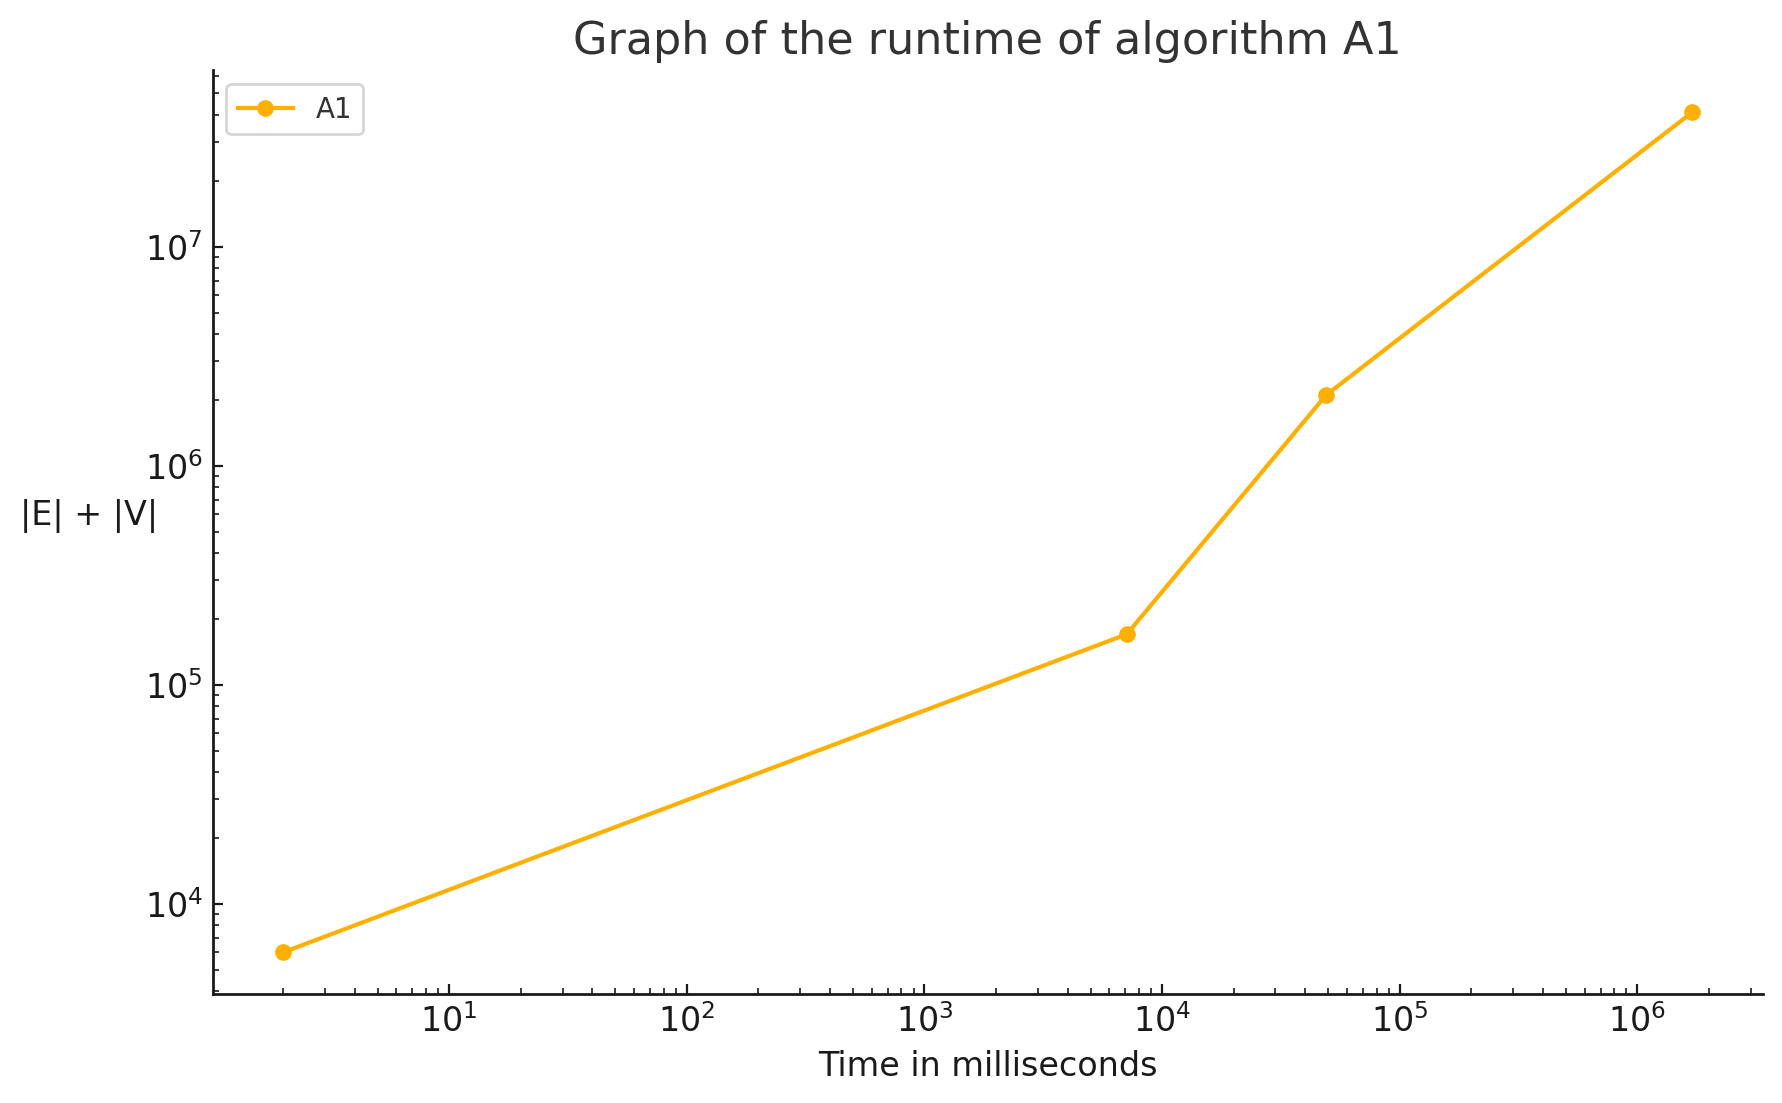
\includegraphics[width=\linewidth]{output (2).png}
  \caption{Graph of the runtime of $A1$ algorithm in milliseconds.}
  \label{fig:100milliseconds}
\end{figure}

The running time of the algorithm A1 depends on both the number of edges and the number of vertices. From the \Cref{fig:100milliseconds} and \Cref{tbl:algorithms} values, it is clear that the algorithm is linear within the tested range.